\section{Numerical radial sequence}\label{sec:sequence}
A width minimum is a numerical candidate; a resolved winding of a
specified two-component matching map adds numerical evidence; an
interval enclosure with analytic tails establishes infinite-domain
existence. Table~\ref{tab:ladder} keeps these levels separate.
The winding concept has a photonic BIC precedent~\cite{Zhen2014}; here
it is applied to a matching map in parameter space, without transferring
the photonic symmetry-based robustness theorem.
The refined matching calculation for indices $6$--$10$ used radial
steps $0.04$ and $0.02$. Its locations interpolate parameter samples
separated by $2.5\times10^{-4}$. For indices $7$--$10$, the small
inter-grid difference ($2.3\times10^{-8}$ or less) is not a validated location error.
The reported interpolation uncertainty is a few $10^{-6}$.
For indices $11$--$14$, the archived linewidth reconstruction used signs
chosen to match neighboring slopes. Those rows remain weaker evidence;
no additional matching calculation was made for this revision.

\begin{table}[htbp]\centering\small
\caption{Radial candidates at $\beta=1/2$. Displayed numerical digits
are not interval enclosures. Certificates C0/C1 are given in
Section~\ref{sec:certified-existence}; the remaining entries are finite-domain
numerical evidence. The last three error estimates are empirical.}
\label{tab:ladder}
\begin{tabular}{rll}\toprule
$n$&$\omega^2$&Evidence\\\midrule
1&$0.797676787\ldots$&Existence enclosure C0\\
2&$0.685128904\ldots$&Existence enclosure C1\\
3&$\sim0.631450$&Resolved numerical winding\\
4&$\sim0.601421$&Resolved numerical winding\\
5&$\sim0.582417$&Sign change; winding unresolved\\
6&$\sim0.569360$&Resolved numerical winding\\
7&$\sim0.559848$&Resolved numerical winding\\
8&$\sim0.552619$&Resolved numerical winding\\
9&$\sim0.546940$&Resolved numerical winding\\
10&$\sim0.542364$&Resolved numerical winding\\
11&$\sim0.53860$&Linewidth reconstruction\\
12&$\sim0.535449$&Linewidth reconstruction\\
13&$\sim0.532772$&Linewidth reconstruction\\
14&$\sim0.530470$&Linewidth reconstruction\\
15&$\sim0.52846934$&Subsequent resolved winding\\
16&$0.52671542\pm2\times10^{-7}$&Resolved winding, final bracket rule failed\\
17&$0.52516277\pm1.3\times10^{-6}$&Resolved winding, final bracket rule failed\\
18&$0.5237875\pm4\times10^{-6}$&Crossing count $+1$; phase unresolved\\\bottomrule
\end{tabular}
\end{table}

The subsequent calculation reproduced index $15$ near $0.5284693357$.
For $16$ and $17$, resolved numerical windings are $+1$ and $-1$.
For $18$, the crossing count and sampled phase winding both give $+1$,
but the maximum phase jump $0.585$ radians fails the resolution rule.
All three miss the prescribed final-bracket acceptance criterion; the
empirical errors include roundoff sensitivity. This unsuccessful
combined acceptance rule is retained, even where individual diagnostics
are informative. There is no certificate or completeness result for
these additional candidates.

\begin{figure}[htbp]\centering
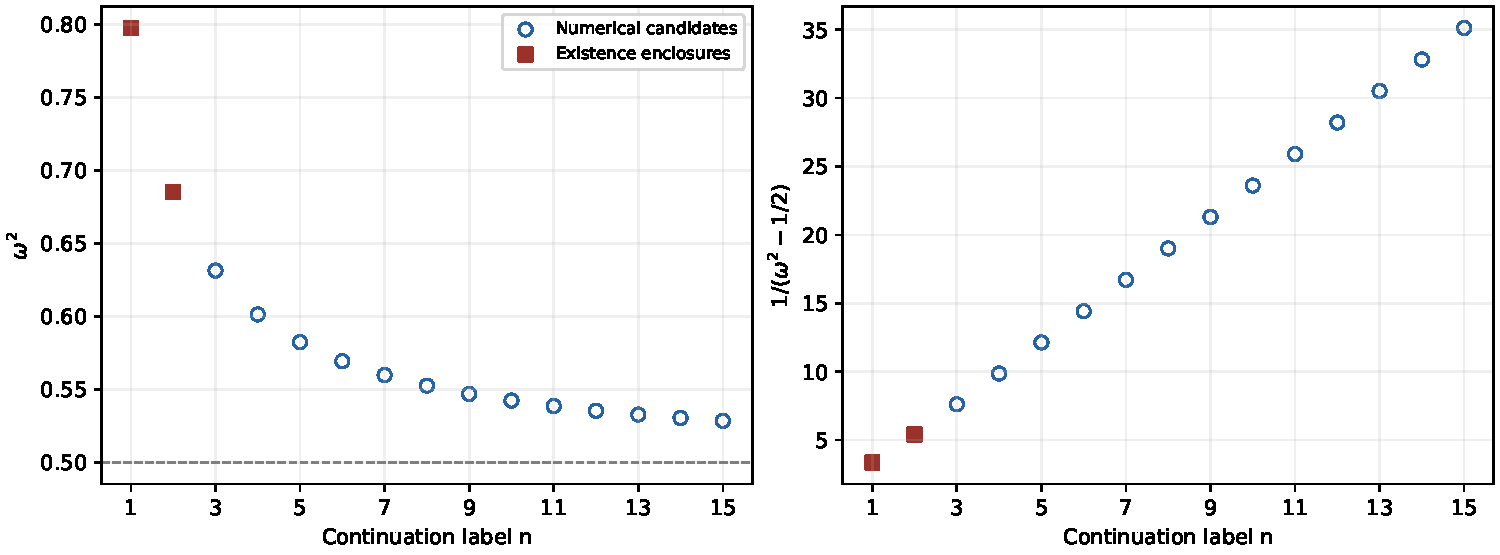
\includegraphics[width=.9\linewidth]{ladder.pdf}
\caption{Archived radial locations through $n=15$ and their inverse
detunings $1/(\omega^2-1/2)$. Filled symbols mark C0/C1. The plot retains
its original fifteen-point dataset, including the earlier rounded
index-$15$ estimate; Table~\ref{tab:ladder} records the subsequent
$15$--$18$ calculation explicitly. The supplementary source inventory
binds the figure to its data. No new fit or extrapolated points are added.}
\label{fig:ladder}
\end{figure}

\paragraph{Prediction history.}\label{sec:predictions}
A sequential extrapolation was updated after each group of targets.
A separate four-parameter thin-wall fit used indices $5,7,8,9$;
its author reported separation from later target values, which were
already known to the coordination team. The frozen file of
30 September 2026, 08:33:26 CEST, and its SHA256 binding are included in
the supplementary source inventory. This is a documented calibrated
extrapolation, not global preregistration. The five later comparisons
passed their respective diagnostic windows, but showed a systematic
thin-wall offset of about $2\times10^{-5}$, comparable to those windows.
The unfitted planar comparison below therefore carries the mechanistic
interpretation; the forecast history does not establish zero linewidth.
